% !TEX root = ../main.tex

\section{Dataset Overview}
\label{schema}

The steps in Section~\ref{dataset} led to the construction of the 
Wonderless Serverless computing dataset, consisting of $1,877$
real-world Serverless applications worthing $44 \, GB$ of data. 

First, a CSV file that contains the URL of each repository. 
With this format one can clone the latest version of the repositories any time. 
On the negative side, the repositories can change access to private, 
be removed entirely, or drop the services related to Serverless computing 
over time. 

To overcome these issues, we provide a snapshot of the 
repositories taken on November 8, 2020. 
In the snapshot, each repository is assigned a directory named `$a\_b$' 
where `$a$' is the GitHub username of the developer and `$b$' is the name of the repository. 
The directories are categorized into eight parts based on the provider of the applications, 
retrieved from the $serverless.yml$ configuration file. 
The categories are AWS, Azure, Google, OpenWhisk, Cloudflare, Kubeless, 
Spotinst, and Other(for providers supporting less than three applications in the dataset).
If an application used multiple providers, we placed the repository across 
all the related groups. 

Wonderless has a total number of $197,993$ files developed in various programming languages. 
We used CLOC\footnote{\url{https://github.com/AlDanial/cloc}} to count the number of files and 
lines of code based on each programming language. Table~\ref{tab:pl} demonstrates these numbers 
together with the occurrence of runtimes specified in configuration files of Serverless applications. 
Based on the applications in the dataset, Nodejs with $\%72.2$ of occurrence is the most popular runtime 
for Serverless applications.

\vspace{-2mm}
\begin{table}[h]
	\begin{center}
		\caption{Distribution of programming languages in Wonderless.}
		\label{tab:pl}
		\begin{tabular}{c|c|c|c}
			\textbf{Language} & \textbf{Files} & \textbf{Lines of Code} & \textbf{\%Occurrence} \\
			\toprule
			JavaScript &  44,279 & 7,332,365 & \multirow{2}{*}{\%72.2} \\
			TypeScript & 22,517 & 1,429,896 &  \\ \midrule
			Python & 15,875 & 2,083,442 & \%19 \\ \midrule
			Java & 11,556 & 415,665 & \%2.7  \\ \midrule
			Ruby & 3,001 & 91,499 & \%0.5  \\ \midrule
			Go & 2,283 & 489,636 & \%2.4 \\ \midrule
			Other & 98,482 & 28,281,135 & \%3.2 \\ \midrule
			Total & 197,993 & 40,123,638 & \%100\\ \midrule
		\end{tabular}
	\end{center}
\end{table}
\vspace{-5mm}

Git history of the applications is included in Wonderless. 
According to the results extracted using \emph{git log}, there are $374,922$ git commits for all the 
applications in the dataset. Overall, $13,984$ developers contributed to these applications while 
more than $\%80$ of the applications have less than five contributors.

\begin{figure}
	\centering
	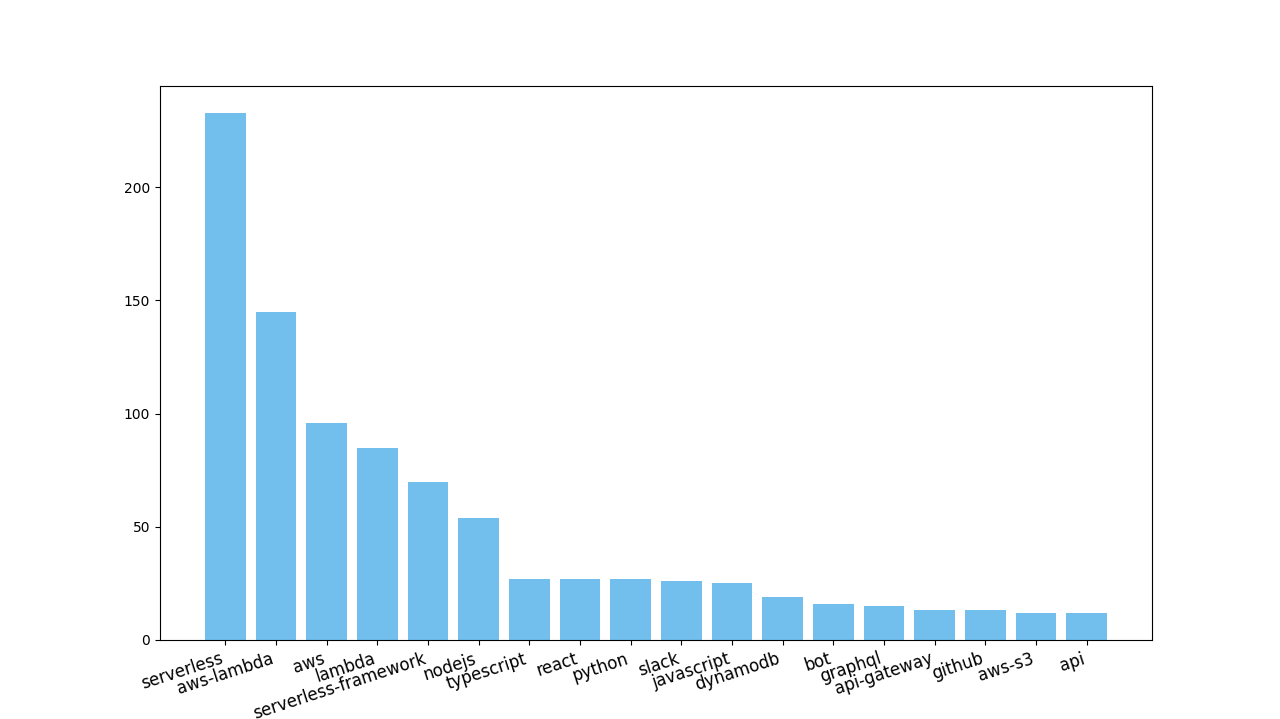
\includegraphics[scale=0.3]{figures/topics.png}
	\caption{Popular topics in Serverless applications.}
	\label{fig:topics}
\end{figure}

We extracted the meta-data of repositories using the \emph{mercy-preview} media 
type of GitHub API previews. Based on this data, $\%46$ of the repositories have a license 
among which $\%67$ are MIT License. More than $\%48$ of the repositories have at least one 
GitHub star while more than $\%96$ of them have less than $100$ stars. Figure~\ref{fig:topics} 
represents the distribution of topics with more than ten occurrences in the dataset.
